% Preamble -------------------------------------------------
\documentclass{beamer}
\usepackage[utf8]{inputenc}
\usepackage[ngerman]{babel}
\usepackage{adjustbox}
\usepackage{tikz}
  \usetikzlibrary{positioning, calc, decorations.pathreplacing, backgrounds, fit}
\usepackage{multirow}
\usepackage{graphicx}
\usepackage{caption}

\definecolor{grey538}{rgb}{240,240,240}

% Slides setup ---------------------------------------------
\usetheme{Berlin}
\usecolortheme{seagull}
\usefonttheme{professionalfonts}

\title{Zusammenfassung vom 11. Dezember 2017}
\author{Dag Tanneberg\thanks{%
  \href{mailto:dag.tanneberg@uni-potsdam.de}%
    {dag.tanneberg@uni-potsdam.de}
  }
}
\institute[Universität Potsdam]{
  {\glqq}Forschungsdesign in den Sozialwissenschaften{\grqq}\\
  Universität Potsdam\\
  Lehrstuhl für Vergleichende Politikwissenschaft\\
  Wintersemester 2017/2018
}
\date{18. Dezember 2017}

\begin{document}
\maketitle

\begin{frame}
\frametitle{Warum messen wir?}
  \textbf{Messen}
  \begin{itemize}
    \item ermöglicht den \textit{pointierten} Vergleich von Objekten
    \item ordnet Objekten Zahlen gemäß festgelegter Regeln zu
    \item strebt strukturtreue Abbildung der Realität an
    \begin{itemize}
      \item [$\rightarrow$] Ordnung der Messergebnisse wahrt empirische Ordnung
    \end{itemize}
  \end{itemize}
  \vfill
  \begin{table}
  \centering
  \begin{tabular}{*{3}{c}|*{3}{c}}
  \multicolumn{3}{c}{richtig} & \multicolumn{3}{c}{falsch}\\
  Objekt & & Messerg. & Objekt & & Messerg. \\\hline
  \color{blue!25}{A} & $\rightarrow$ & \color{blue!25}{1} & \color{blue!25}{A} & $\rightarrow$ & \color{blue!100}{3}\\
  \color{blue!63}{B} & $\rightarrow$ & \color{blue!63}{2} & \color{blue!63}{B} & $\rightarrow$ & \color{blue!25}{1}\\
  \color{blue!100}{C} & $\rightarrow$ & \color{blue!100}{3} & \color{blue!100}{C} & $\rightarrow$ & \color{blue!63}{2}\\
  \end{tabular}
  \end{table}
\end{frame}

\begin{frame}
  \frametitle{Welche Eigenschaften haben Messergebnisse?}
  \textbf{Skalentyp/-niveau}
  \begin{itemize}
    \item fasst Eigenschaften eines Messergebnisses zusammen
    \item informiert über den Informationsgehalt einer Messung
    \item [$\rightarrow$] informativere Messungen erlauben mehr Anwendungen
  \end{itemize}
  \vfill
  \begin{table}
    \footnotesize
    \centering
    \caption*{Festgelegte Eigenschaften der wichtigsten Skalentypen}
    \begin{tabular}{l*{5}{c}}
                           & Nominal    & Ordinal    & Intervall   & Ratio\\ \hline
      Distinkte Kategorien & \checkmark & \checkmark & \checkmark & \checkmark \\
      Geordnete Kategorien &            & \checkmark & \checkmark & \checkmark \\
      Gleiche Abstände     &            &            & \checkmark & \checkmark \\
      Absoluter Nullpunkt  &            &            &            & \checkmark \\
      Beispiel & Gender & Gefahrenlage & $^{\circ}$C & Länge\\\hline
    \end{tabular}
  \end{table}
  \vfill
\end{frame}

\begin{frame}
\frametitle{Gütekriterien einer Messung}
  \begin{columns}
    \begin{column}{.5\textwidth}
      \begin{figure}
        \caption*{\textbf{Reliabilität}}
        \begin{tikzpicture}[
          grow = right, edge from parent/.style={draw,-latex},
          level distance = 8em, sibling distance = 8em, minimum size = 2em, inner sep = 0,
          scale = 1.5,
          background rectangle/.style = {fill = gray!10},%
          show background rectangle
        ]
          \tikzstyle {latent} = [draw, shape = circle, fill = white]
          \tikzstyle {observed} = [draw, shape = rectangle, fill = white]
          % place nodes
          \path node (0) [latent] at (0,0) {$\theta$};
          \path node (1) [observed] at (1,0) {$x$};
          \path node (2) [latent] at (1,1) {$\epsilon$};
          % place edges
          \foreach \x in {0, 2}
            { \draw [-latex] (\x) -- (1) ; } ;
          \begin{scope}[on background layer]
            \node [fill=grey538, fit = (0) (1) (2)] {};
          \end{scope}
        \end{tikzpicture}
      \end{figure}
      \begin{itemize}
        \item Zuverlässigkeit d. Messung
        \item schwankt d. Zufallseinflüsse
        \item erford. standard. Messung
      \end{itemize}
    \end{column}
    \begin{column}{.5\textwidth}
      \begin{figure}
        \caption*{\textbf{Validität}}
        \begin{tikzpicture}[
          grow = right, edge from parent/.style={draw,-latex},
          level distance = 8em, sibling distance = 8em, minimum size = 2em, inner sep = 0,
          scale = 1.5,
          background rectangle/.style = {fill = gray!10},%
          show background rectangle
        ]
          \tikzstyle {latent} = [draw, shape = circle, fill = white]
          \tikzstyle {observed} = [draw, shape = rectangle, fill = white]
          % place nodes
          \path node (0) [latent] at (0,0) {$\theta$};
          \path node (1) [observed] at (1,0) {$x$};
          \path node (2) [observed, inner sep = 1] at (.5,1) {Drittvariable};
          % place edges
          \foreach \x in {0, 1}
            { \draw [-latex] (2) -- (\x) ; } ;
          \draw [-latex, ] (0) [dashed] to (1) ;
          \begin{scope}[on background layer]
            \node [fill=grey538, fit = (0) (1) (2)] {};
          \end{scope}
        \end{tikzpicture}
      \end{figure}
      \begin{itemize}
        \item Gültigkeit d. Messung
        \item leidet u. system. Störgrößen
        \item erford. starke Theorie
      \end{itemize}
    \end{column}
  \end{columns}
\end{frame}

\begin{frame}
  \frametitle{Wie hängen Reliabilität und Validität zusammen?}
  \begin{columns}
  \begin{column}{.5\textwidth}
    \textbf{Reliabilität und Validität}
    \begin{itemize}
      \footnotesize
      \item fokussieren andere Fehlerquellen
      \item variieren unabhängig voneinander
    \end{itemize}
    \textbf{Validität einer Messung}
    \begin{itemize}
      \footnotesize
      \item hat i.\,d.\,R. Vorrang
      \item erfordert Mindestmaß Reliabilität
      \item [$\rightarrow$] R. notwendige Bdg. für Validität
    \end{itemize}
  \end{column}
  \begin{column}{.5\textwidth}
    \begin{figure}
      \centering
      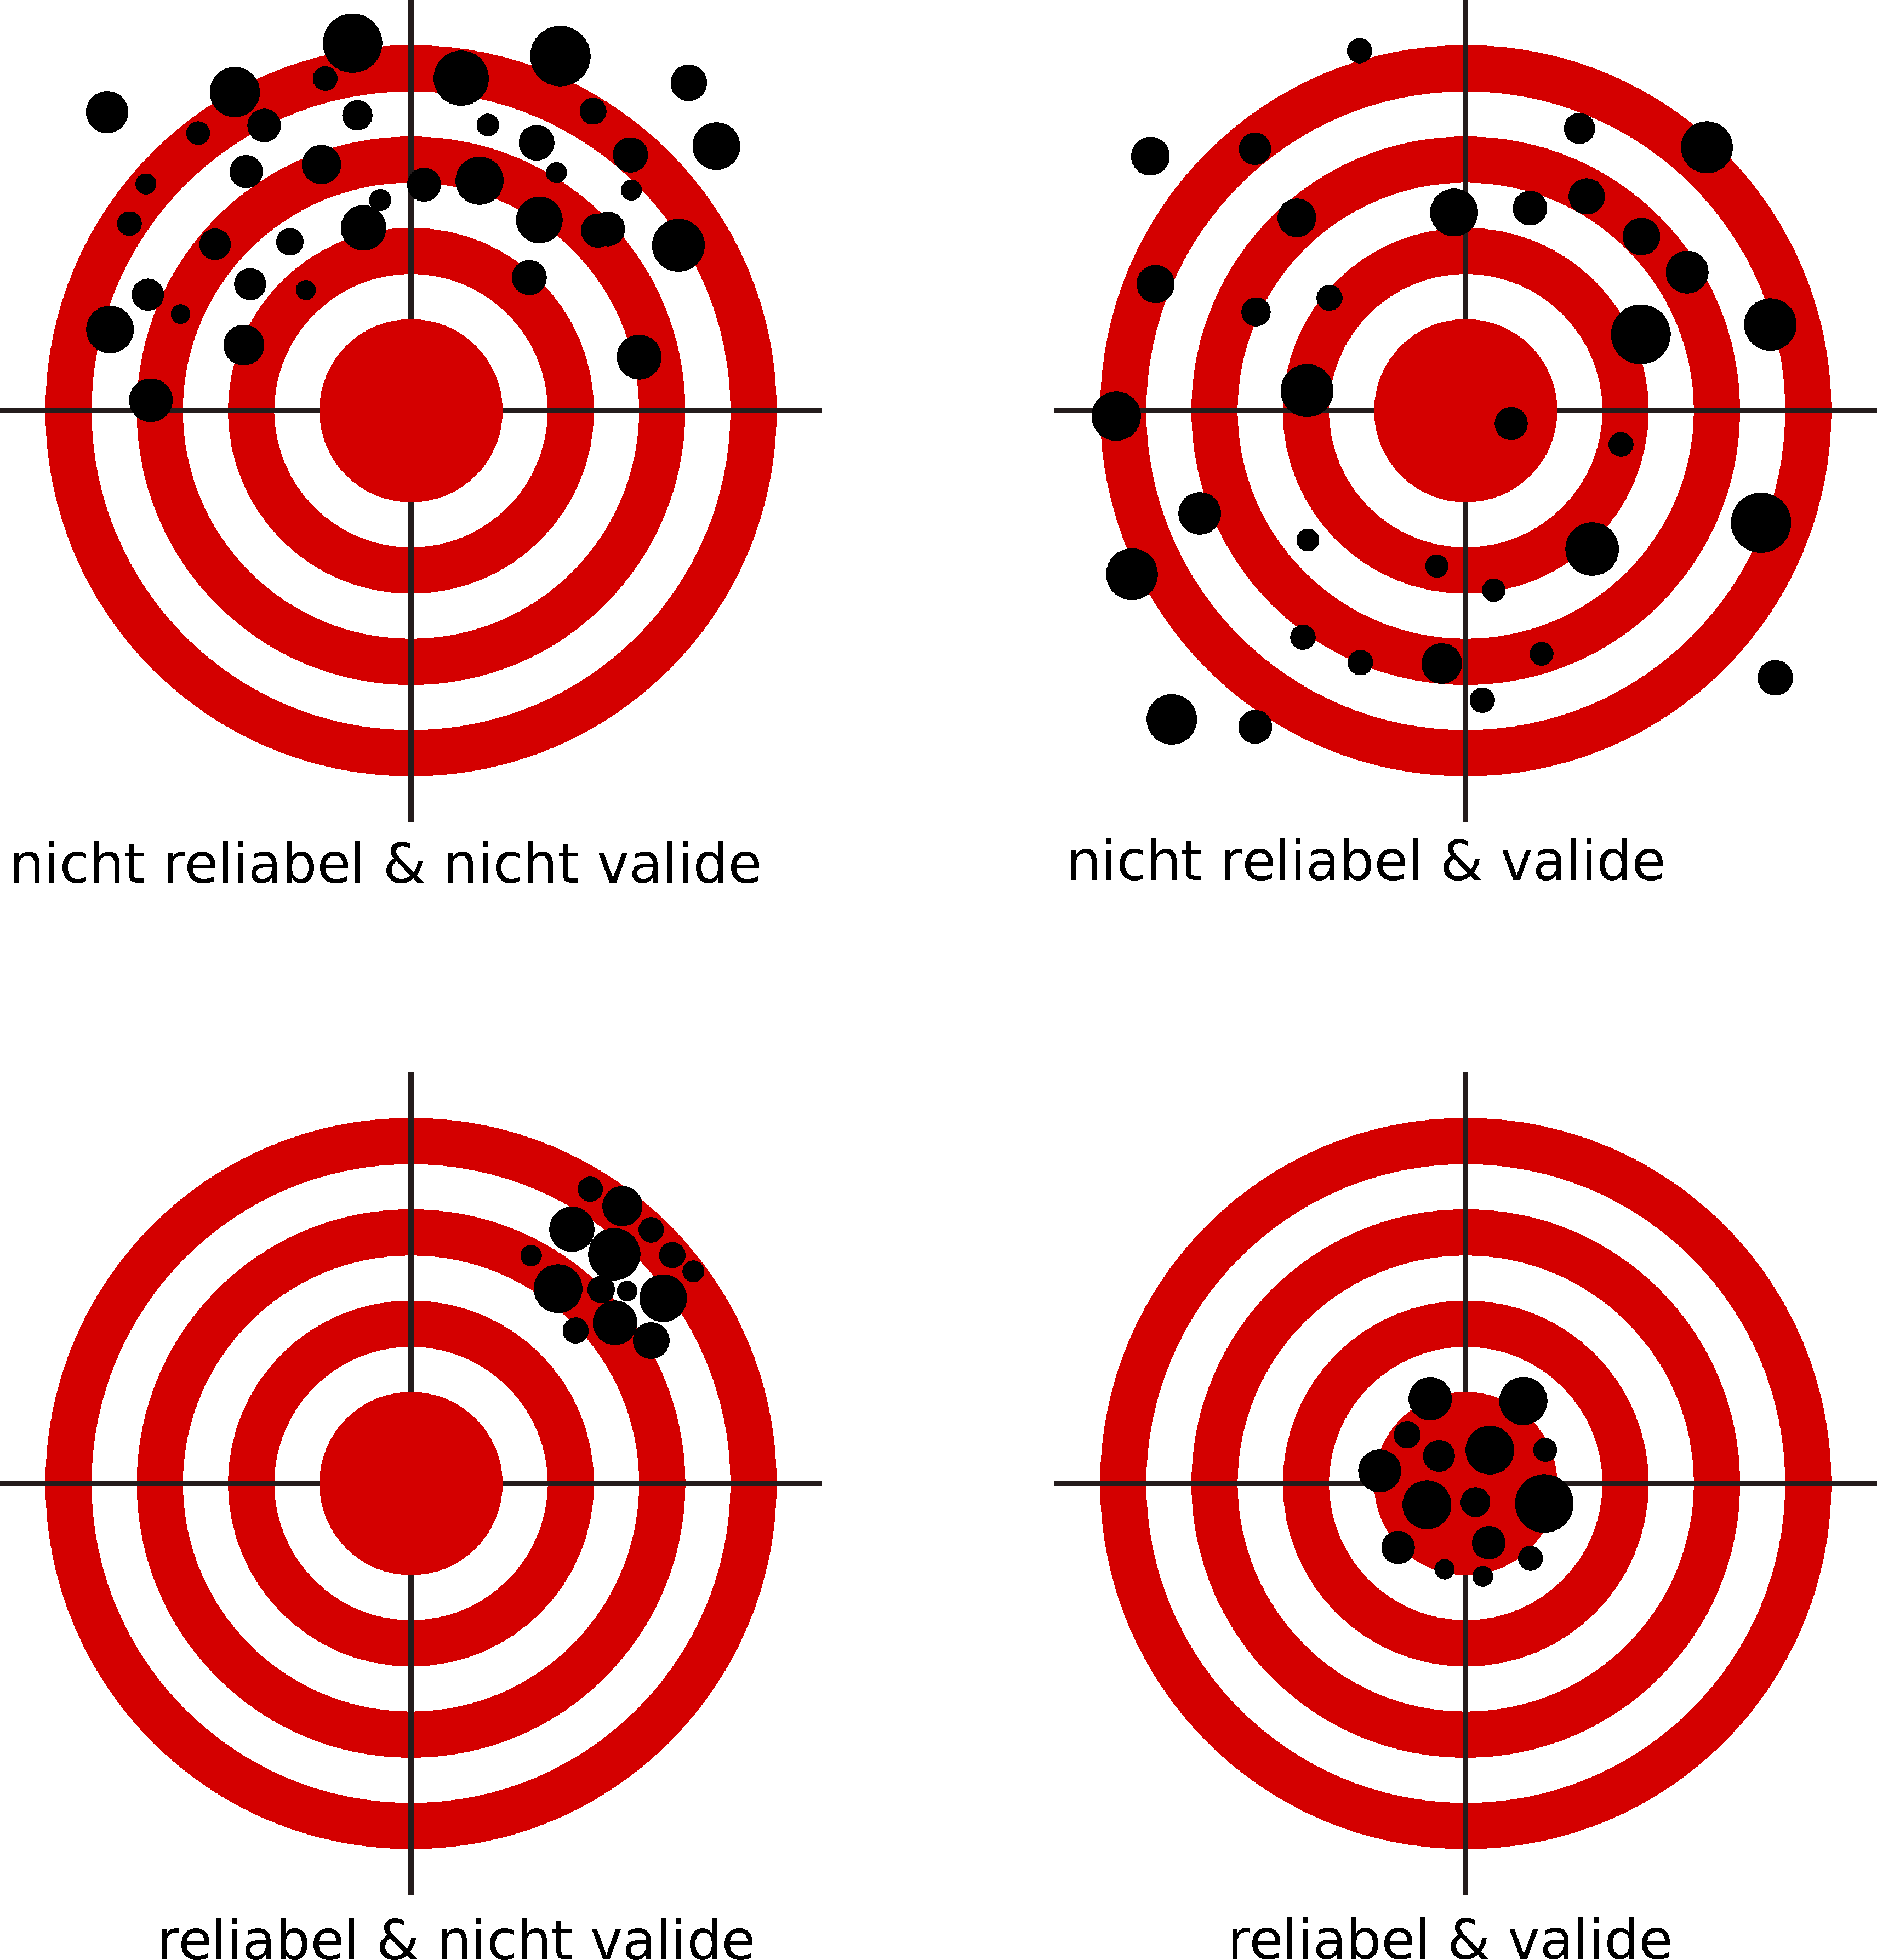
\includegraphics[scale = .09]{Reliability_and_validity_DE.pdf}
    \end{figure}
  \end{column}
  \end{columns}
\end{frame}

\begin{frame}
  \frametitle{Warum fällt den Sozialwiss. gutes Messen so schwer?}
  \begin{enumerate}
    \item Latente Konstrukte
    \begin{itemize}
      \item wichtige Phänomene nicht direkt beobachtet (Frieden)
      \item {\glqq}vereinbarte{\grqq} (kausale) Beziehung zw. Indikator \& Konstrukt
      \item [$\rightarrow$] Messen ist ein theoretischer Akt
    \end{itemize}
    \item Kausale Beziehungen zw. Konstrukt \& Indikator
    \begin{itemize}
      \item reflektive Indik.: latentes Konstrukt verursacht Messwert
      \item formative Indik.: Indikatoren verursachen latentes Konstrukt
      \item [$\rightarrow$] Kausalbeziehung i.\,e.\,S. nicht manipulier- oder prüfbar
    \end{itemize}
    \item Zweckabhängigkeit des Messens
    \begin{itemize}
      \item Differenzierung: möglichst feine Abstufungen zw. Objekten
      \item Gruppierung: Einordnung von Objekten in diskrete Kategorien
      \item [$\rightarrow$] verlangen je eigene Gütekriterien
    \end{itemize}
  \end{enumerate}
\end{frame}
\end{document}